%%%%%%%%%%%%%%%%%%%%%%%%%%%%%%%%%%%%%%%%%
% Beamer Presentation
% LaTeX Template
% Version 1.0 (10/11/12)
%%%%%%%%%%%%%%%%%%%%%%%%%%%%%%%%%%%%%%%%%

%----------------------------------------------------------------------------------------
%	PACKAGES AND THEMES
%----------------------------------------------------------------------------------------

\documentclass{beamer}

\mode<presentation> {

% The Beamer class comes with a number of default slide themes
% which change the colors and layouts of slides. Below this is a list
% of all the themes, uncomment each in turn to see what they look like.

%\usetheme{default}
%\usetheme{AnnArbor}
\usetheme{Antibes}
%\usetheme{Bergen}
%\usetheme{Berkeley}
%\usetheme{Berlin}
%\usetheme{Boadilla}
%\usetheme{CambridgeUS}
%\usetheme{Copenhagen}
%\usetheme{Darmstadt}
%\usetheme{Dresden}
%\usetheme{Frankfurt}
%\usetheme{Goettingen}
%\usetheme{Hannover}
%\usetheme{Ilmenau}
%\usetheme{JuanLesPins}
%\usetheme{Luebeck}
%\usetheme{Madrid}
%\usetheme{Malmoe}
%\usetheme{Marburg}
%\usetheme{Montpellier}
%\usetheme{PaloAlto}
%\usetheme{Pittsburgh}
%\usetheme{Rochester}
%\usetheme{Singapore}
%\usetheme{Szeged}
%\usetheme{Warsaw}

% As well as themes, the Beamer class has a number of color themes
% for any slide theme. Uncomment each of these in turn to see how it
% changes the colors of your current slide theme.

%\usecolortheme{albatross}
%\usecolortheme{beaver}
%\usecolortheme{beetle}
%\usecolortheme{crane}
%\usecolortheme{dolphin}
%\usecolortheme{dove}
%\usecolortheme{fly}
%\usecolortheme{lily}
%\usecolortheme{orchid}
%\usecolortheme{rose}
%\usecolortheme{seagull}
%\usecolortheme{seahorse}
%\usecolortheme{whale}
%\usecolortheme{wolverine}

%\setbeamertemplate{footline} % To remove the footer line in all slides uncomment this line
%\setbeamertemplate{footline}[page number] % To replace the footer line in all slides with a simple slide count uncomment this line

%\setbeamertemplate{navigation symbols}{} % To remove the navigation symbols from the bottom of all slides uncomment this line
}
%\usepackage{beamerthemeshadow}
\usepackage{graphicx} % Allows including images
%\usepackage{booktabs} % Allows the use of \toprule, \midrule and
\usepackage[brazil]{babel}
\usepackage[T1]{fontenc}
\usepackage[utf8]{inputenc}
\usepackage{amsthm,amsfonts,amssymb,amsxtra,empheq}
\usepackage{bm,amsmath,latexsym}
\usepackage{verbatim}
\usefonttheme[onlymath]{serif} % fonte modo matematico
%\renewcommand\mathfamilydefault{\rmdefault} % modo default modo matematico
\usepackage{animate}

\setbeamertemplate{theorems}[numbered]
\theoremstyle{plain}
\newtheorem{exem}{Exemplo}
\newtheorem{teo}{Teorema}
\newtheorem{mot}{Motivação}
\newtheorem{defi}{Definição}
\newcommand{\iid}{\stackrel{\mathrm{iid}}{\sim}}

%----------------------------------------------------------------------------------------
%	TITLE PAGE
%----------------------------------------------------------------------------------------

\title[Esperança, Variância e Esperança condicional]{Esperança, Variância e Esperança condicional} % The short title appears at the bottom of every slide, the full title is only on the title page

\author{Ben D\^eivide} % Your name
\institute[UFLA] % Your institution as it will appear on the bottom of every slide, may be shorthand to save space
%{
%UFLA \\ % Your institution for the title page
%\medskip
%\textit{ben.deivide@gmail.com}\\ % Your email address
%\textit{www.benalana.blogspot.com}
%}
%\date{\today} % Date, can be changed to a custom date

\begin{document}

\begin{frame}
\titlepage % Print the title page as the first slide
\end{frame}

\begin{frame}
\frametitle{Sumário} % Table of contents slide, comment this block out to remove it
\tableofcontents % Throughout your presentation, if you choose to use \section{} and \subsection{} commands, these will automatically be printed on this slide as an overview of your presentation
\end{frame}

%----------------------------------------------------------------------------------------
%	PRESENTATION SLIDES
%----------------------------------------------------------------------------------------

%------------------------------------------------

\section{Noções Sobre Valor Esperado ou Esperança Matemática e Variância}

  \begin{frame}
    \frametitle{Valor Esperado e Variância}
    \begin{itemize}
    	\item Variável Aleatória discreta $X$ $\Rightarrow$ $S_X = \{x_1, x_2, \ldots, x_N\}$;\pause
    	\item $P(X = x_i) = 1/N$;\pause
    	\item $x_1 \times \frac{1}{N} + x_2 \times \frac{1}{N} + \ldots + x_N \times \frac{1}{N} = \frac{1}{N}\sum_{i = 1}^{N}x_i = \bar{x}_N$;\pause
    	\item $x_1 \times p_1 + x_2 \times p_2 + \ldots + x_N \times p_N = \sum_{i = 1}^{N}x_ip_i$ (Valor Esperado)\pause
    	\item Valor esperado ou Esperança matemática como medida de locação e Variância como medida de dispersão ou forma (No R!);
    \end{itemize}
  \end{frame}
  
  \section{Esperança matemática e suas propriedades}
  
  \begin{frame}
  	\frametitle{Esperança matemática}
  	\begin{itemize}
  		\item Variável Aleatória discreta $X$ $\Rightarrow$ $S_X = \{x_1, x_2, \ldots, x_N\}$;\pause
  		\item $P(X = x_i) = 1/N$;\pause
  		\item $x_1 \times \frac{1}{N} + x_2 \times \frac{1}{N} + \ldots + x_N \times \frac{1}{N} = \frac{1}{N}\sum_{i = 1}^{N}x_i = \bar{x}_N$;\pause
  		\item $x_1 \times p_1 + x_2 \times p_2 + \ldots + x_N \times p_N = \sum_{i = 1}^{N}x_ip_i$ (Valor Esperado)\pause
  		\item Valor esperado ou Esperança matemática como medida de locação e Variância como medida de dispersão ou forma (No R!);
  	\end{itemize}
  \end{frame}
  
  \begin{frame}
  	\frametitle{Esperança matemática}
  	\begin{defi}[Esperança matemática]\label{def:esperanca}
  		Seja $X$ uma variável aleatória em $(\Omega,\mathcal{F},P)$. A esperança matemática (ou média) de $X$, denotada por $\mu_X$ ou $E[X]$, é definida:
  		\begin{enumerate}[i)]
  			\item se $X$ for discreta,
  			\begin{equation}
  			E[X] = \sum_x x P_X(x),
  			 \end{equation}
  			\item se $X$ for contínua,
  			\begin{equation}
  			E[X] = \int^{\infty}_{-\infty} x f_X(x)dx.
  			\end{equation}
  		\end{enumerate}
  	\end{defi}
  \end{frame}
  
   \begin{frame}
   	\frametitle{Propriedades da Esperança matemática}
   	
   \end{frame}
  
  
\section{Esperança condicional}

\begin{frame}
	\frametitle{Problema dos tetraedros}
    Um experimento com dois tetraedros deseja observar o número da face superior desses tetraedros. Denote $X$ como o número da face superior do primeiro tetraedro e $Y$ o maior número da face superior desses dois tetraedros. O Espaço amostral é dado por:
    \begin{align*}
    \Omega = & \{(1,1), (1,2), (1,3), (1,4), \\
    & (2,1), (2,2), (2,3), (2,4), \\
    & (3,1), (3,2), (3,3), (3,4), \\
    & (4,1), (4,2), (4,3), (4,4)\}
    \end{align*}\pause
    Os valores que $(X, Y)$ podem assumir são:
    \begin{align*}
    (X, Y) = & \{(1,1), (1,2), (1,3), (1,4), (2,2), \\
             & (2,3), (2,4),(3,3), (3,4), (4,4)\}
    \end{align*}
\end{frame}

\begin{frame}
	\frametitle{Problema dos tetraedros}
	A função de probabilidade conjunta é dada por:
	\begin{center}
		\tiny
		\begin{tabular}{|c|c|c|c|c|c|c|c|c|c|c|}
			\hline
			$(x,y)$ & $(1, 1)$ & $(1,2)$ & $(1,3)$ & $(1,4)$ & $(2,2)$ \\
			\hline
			$P_{X, Y}(x,y)$ & $\frac{1}{16} = 0,0625$ &  $\frac{1}{16}$ & $\frac{1}{16}$ & $\frac{1}{16}$ & 
			$\frac{2}{16} = 0,125$ \\
			\hline
			\hline
			$(x,y)$ & $(2,3)$ & $(2,4)$ & $(3,3)$ & $(3,4)$ & $(4,4)$\\
			\hline
			$P_{X, Y}(x,y)$ & $\frac{1}{16}$ & $\frac{1}{16}$ & $\frac{3}{16} = 0,1875$ & $\frac{1}{16}$ & $\frac{4}{16} = 0,25$\\
			\hline
		\end{tabular}
		
		\begin{center}
			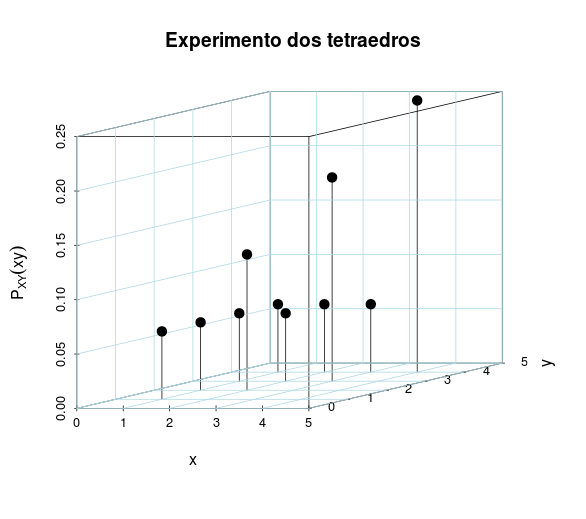
\includegraphics[scale = 0.3]{exptetraedros}
			
		\end{center}
	\end{center}
\end{frame}

\begin{frame}
	\frametitle{Problema dos tetraedros}
	Gráfico da Função de Probabilidade conjunta $P_{X, Y}$
	 \begin{center}
	 	\animategraphics[controls, loop, width=0.7\textwidth]{4}{plot3d/tet}{1}{71}
	 \end{center}
\end{frame}

\begin{frame}
	\frametitle{Problema de variáveis aleatórias contínuas}
      \begin{center}
      \begin{center}
      	\animategraphics[controls, loop, width=0.7\textwidth]{10}{plot3dens2/dens3d}{1}{307}
      \end{center}
       \end{center}
\end{frame}


\end{document} 